\begin{problem}[09]
求盛水容器底侧的小孔出流速度.
\end{problem}
% --------------------------------------------------------------------
\begin{solution}
\begin{minipage}[c]{0.8\linewidth}
小孔出流是一个纯粹的力学问题, 与容器中水的高度$h$, 重力加速度$g$和小孔的直径$d$有关, 小孔出流速度为$v$, 则有
\[
v = f(d, g, h)
\]
\end{minipage}
\begin{minipage}[c]{0.2\linewidth}
\begin{center}
\usetikzlibrary{%
    decorations.pathreplacing,%
    decorations.pathmorphing,arrows
}
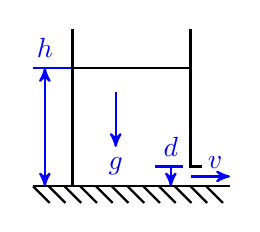
\begin{tikzpicture}[ media/.style={font={\footnotesize\sffamily}},
    wave/.style={
        decorate,decoration={snake,post length=1.4mm,amplitude=2mm,
        segment length=2mm},thick},
    interface/.style={
        postaction={draw,decorate,decoration={border,angle=-45,
                    amplitude=0.3cm,segment length=2mm}}}]
\draw[thick,interface](-1.25,0)--(1.25,0);
\draw[thick] (-0.75,0) -- (-0.75,2);
\draw[thick] (0.9,0.25)--(0.75,0.25) -- (0.75,2);

\draw[thick,->,>=stealth',blue] (0.75,0.125)--(1.25,0.125) node[above left=-1pt]{$v$};

\draw[thick](-0.75,1.5)--(0.75,1.5);
\draw[thick,blue](-0.77,1.5)--(-1.25,1.5);
\draw[ <->,>=stealth',thick,blue](-1.1,0) -- (-1.1,1.5) node[above]{$h$};

\draw[thick,blue](0.3,0.25) -- (0.65,0.25);
\draw[ <-,>=stealth',thick,blue](0.5,0) -- (0.5,0.25) node[above]{$d$};


\draw [blue,->,>=stealth',thick] (-0.2,1.2) -- (-0.2, 0.5) node [below]{$g$};
\end{tikzpicture}
\end{center}
\end{minipage}
上式中各物理量的量纲分别为:$[v]=LT^{-1}$, $[d]=L$, $[g]=LT^{-2}$, $[h]=L$, 取$h,g$为基本量, 且作为本问题的单位系统, 用以度量问题中的各量, 于是上式转化为
\[
\frac{v}{\sqrt{gh}}=f\bigg(\frac{d}{h},1,1\bigg)=f\bigg(\frac{d}{h}\bigg)
\]
由于小孔有$d\ll h$, 则有$d/h\rightarrow 0$, 所以$f(d/h)=f(0)=C$, 因此小孔出流速度为
\[
v = C\sqrt{gh}
\]
其中$C$为常数, 可进一步由理论确定$C=\sqrt{2}$.
\end{solution}
